\subsection{Password checking}
\label{sec:PASS_CHECK}

Once every digit has been checked individually, all of them have to be checked to determine whether the whole password is correct or not. To do this, we will make use of another GAL, namely \textit{PASSWORD CHECK}.
\medskip

The latter has as an input, the clock (\textit{CLK}), \textit{DONE\_}, which is the delayed version of DONE (See \textbf{Subsection \ref{sec:DELAYED_STEADY}}), the 4 \textit{DIGIT\_} signals coming from the individual checks and the general \textit{RESET}. As outputs, it has \textit{CORRECT} signal, and \textit{SENT\_PULSE\_}, a signal that is used to initialize the time-sensitive operations which purpose is to display the introduced password in the 4 7-segment displays followed by the \textbf{\textit{Open}}/\textbf{\textit{Error}} message and finally, once everything has been displayed, to reset the whole circuit.\medskip

The \textit{DONE\_} signal is a slighty delayed version of the original \textit{DONE} signal. This is needed because otherwise the individual digit signals, which are normally LOW, arrive \textbf{AFTER} the \textit{DONE} one, creating a point in time in which the \textit{DONE} is \textbf{HIGH}, which would indicate that the password has been entered, but the \textit{DIGIT\_} signals are still \textbf{LOW} since the GALs in \textbf{Subsection \ref{sec:IND_CHECK}} have not had the time to process the digits yet. Delaying the \textit{DONE} signal by some ms, a time higher than the propagation delay of the GALs, solves this problem.\bigskip

We will now go over all the states that form the FSM:

\medskip
    \bm{$Q_0$}
\medskip

The code follows the operation of a FSM with 3 states. In \textit{$Q_0$}, \textit{CORRECT} and \textit{SENT\_PULSE} are initialized as LOW level, and remain in this condition until a HIGH is read in the delayed version of \textit{DONE}, \textit{DONE\_}. Depending on the value of \textit{DIGIT\_} in that moment, the next state will either be \textit{$Q_1$} or \textit{$Q_2$}.\medskip

If all bits of the \textit{DIGIT\_} array are on a HIGH level, it means that every digit stored in the RAM coincides in magnitude and order to the ones stored in the dip switches inside the security box. In this case the next state is \textit{$Q_1$}.\medskip

On the other hand, if all bits of the \textit{DIGIT\_} array are NOT on a HIGH level, the state will change to \textit{$Q_2$}. 

\medskip
    \bm{$Q_1$}
\medskip

If the GAL is in this state, it will pull \textbf{\textit{CORRECT}} and \textbf{\textit{SENT\_PULSE}} \textbf{HIGH} and it will wait for the \textit{RESET} signal. Once received, the state will toggle to \textit{$Q_0$} effectively resetting the GAL.

\medskip
    \bm{$Q_2$}
\medskip

In this state the GAL will pull the \textbf{\textit{CORRECT}} signal \textbf{LOW}, so as to indicate that it is NOT correct, and it will pull the \textbf{\textit{SENT\_PULSE}} \textbf{HIGH}, initializing the time-sensitive sequence that we discussed earlier. As per the last state, when a HIGH is received in the \textit{RESET} pin, the state will toggle to \textit{$Q_0$} effectively resetting the GAL.

\clearpage

To illustrate the different states and the transitions between them we have included the following diagram:

\begin{figure}[H]
    \centering
    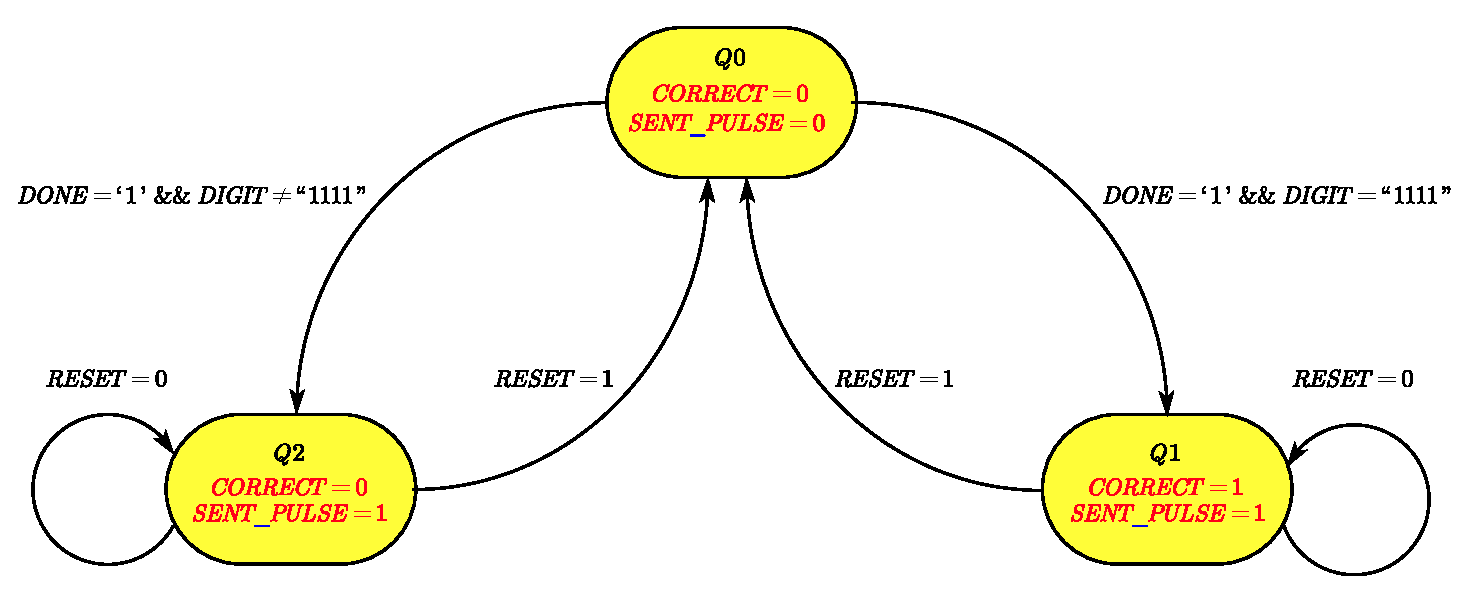
\includegraphics[scale = 0.55]{Graphics/PASSWORD CHECK/PASSWORD_CHECK_FSM.pdf}
    \caption{Password Check FSM}
    \label{fig:PASSWORD_CHECK_FSM}
\end{figure}

\vspace{0.5cm}

The VHDL code describing the operation of the FSM is attached below:

\inputcode{Code/MULTIPLIER.vhd}

Finally, the Proteus subassembly of the circuit can be found below:

\begin{figure}[H]
    \centering
    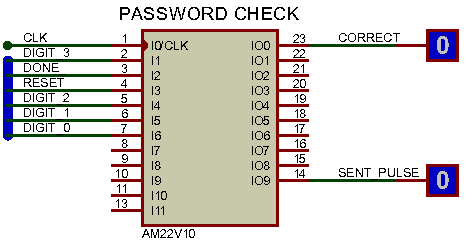
\includegraphics[scale = 1]{Graphics/PASSWORD CHECK/PASSWORD_CHECK_PROTEUS.PDF}
    \caption{Proteus Subassembly of Password Check}
    \label{fig:PASSWORD_CHECK_PROTEUS}
\end{figure}